\section{Auswertung}
\label{sec:Auswertung}
Die in \autoref{sec:Auswertung} gezeigten Grafiken und Rechnungen sind mithilfe der Python-Bibliotheken Matplotlib \cite{matplotlib}, Scipy \cite{scipy} und Numpy \cite{numpy}
erstellt worden.

\subsubsection{Bestimmung der Elementarladung}
Die Messwerte sind in \autoref{tab:messwerte} zu sehen. Bei lückenhaften Messreihen wurden die fehlenden Werte durch den zuvor gemessenen Wert ersetzt, um die Verarbeitung der Daten zu vereinfachen.
\begin{table}[H]
  \centering
  \caption{Messwerte der Messreihe 1.}
  \label{tab:messwerte}
  \begin{tabular}{c | c | c | c | c | c | c | c }
    \toprule
    {$t_0\,/\symup{s}$} & {$t_{auf,1}\,/\symup{s}$} & {$t_{auf,2}\,/\symup{s}$} & {$t_{auf,3}\,/\symup{s}$} & {$t_{ab,1}\,/\symup{s}$} & {$t_{ab,2}\,/\symup{s}$} & {$t_{ab,3}\,/\symup{s}$} & {$R\,/\symup{M \Omega}$} \\
    \midrule
    62.43 & 4.16 & 4.71 & 2.54 & 3.66 & 3.50 & 1.5 & 2.064 \\
    23.75 & 3.63 & 1.50 & 2.15 & 2.68 & 1.41 & 2.47 & 2.046 \\
    10.80 & 3.10 & 5.33 & 7.74 & 2.26 & 2.72 & 5.23 & 2.040 \\
    15.75 & 3.18 & 4.02 & 7.72 & 3.25 & 3.63 & 4.08 & 2.029 \\
    16.24 & 6.06 & 6.06 & 6.06 & 10.05 & 10.05 & 10.05 & 2.029 \\
    20.14 & 16.79 & 16.79 & 16.79 & 5.73 & 5.73 & 5.73 & 2.007 \\
    50.90 & 3.16 & 4.17 & 4.17 & 3.35 & 3.35 & 3.35 & 2.007 \\
    47.75 & 2.34 & 3.21 & 3.28 & 2.60 & 2.09 & 2.56 & 1.968 \\
    19.10 & 7.52 & 4.85 & 4.89 & 4.47 & 3.34 & 3.42 & 1.950 \\
    13.64&9.37&9.37&9.37&2.88&2.88&2.88&1.950\\
    18.3&2.52&4.4&3.54&3.29&2.95&2.14&1.931\\
    11.72&12.72&15.07&13.69&3.9&3.58&3.77&1.931\\
    22.01&7.47&6.43&6.31&4.33&4.55&4.77&1.931\\
    19.09&3.77&4.03&3.81&2.8&2.25&2.73&1.931\\
    7.84&5.55&5.55&5.55&4.45&4.45&4.45&1.911\\
    16.11&11.69&19.62&24.73&5.75&6.58&9.1&1.904\\
    10.85&3.92&4.12&4.24&2.44&2.53& 2.26&1.900\\
    13.74&2.99&3.23&3.41&1.98&2.2&2.33&1898\\
    18.85&13.93&9.62&10.13&5.20&5.1&5.09&1.874\\
    \bottomrule
  \end{tabular}
\end{table}
Die gemessenen Zeiten werden nun mit $s = \SI{0.5(0.1)}{\milli\meter}$ in die Geschwindigkeiten umgerechnet und anschließend gemittelt, indem
der Mittelwert der drei Auf- und Abwärtsgeschwindigkeiten gebildet wird.
Zuerst muss überprüft werden, ob die Ladung der Öltröpfchen während der Messung konstant bleibt. Dazu werden nur die Messwerte betrachtet, bei 
denen
\begin{equation*}
  0.5 < 2\frac{v_0}{v_{ab}-v_{auf}} < 1.5
\end{equation*}
gilt.
Die Werte, die diese Bedingung erfüllen, sind in \autoref{tab:bedingung} zu sehen.
\begin{table}[H]
  \centering
  \caption{Messwerte, die die Bedingung erfüllen.}
  \label{tab:bedingung}
  \begin{tabular}{c | c}
    \toprule
    {$v_{auf}\,/\symup{\frac{m}{s}}$} & {$v_{ab}\,/\symup{\frac{m}{s}}$}\\
    \midrule
    $\SI{2.97(0.59)e-05}{}$ & $\SI{8.72(1.74)e-05}{}$ \\
    $\SI{1.30(0.26)e-04}{}$ & $\SI{1.49(0.29)e-04}{}$ \\
    $\SI{1.69(0.34)e-04}{}$ & $\SI{2.06(0.41)e-04}{}$ \\
    $\SI{8.69(1.76)e-05}{}$ & $\SI{1.33(0.26)e-04}{}$ \\
    $\SI{5.33(1.06)e-05}{}$ & $\SI{1.73(0.34)e-04}{}$ \\
    $\SI{3.61(0.72)e-05}{}$ & $\SI{1.33(0.26)e-04}{}$ \\
    $\SI{7.42(1.48)e-05}{}$ & $\SI{1.09(0.21)e-04}{}$ \\
    $\SI{1.29(0.25)e-04}{}$ & $\SI{1.92(0.38)e-04}{}$ \\
    $\SI{2.67(0.55)e-05}{}$ & $\SI{7.00(1.41)e-05}{}$ \\
    $\SI{1.22(0.24)e-04}{}$ & $\SI{2.07(0.41)e-04}{}$ \\
    $\SI{1.56(0.31)e-04}{}$ & $\SI{2.30(0.46)e-04}{}$ \\
    $\SI{4.45(0.90)e-05}{}$ & $\SI{9.74(1.95)e-05}{}$ \\
    \bottomrule
  \end{tabular}
\end{table}

Die Fehler der Geschwindigkeiten ergeben sich mit dem Standardfehler des Mittelwertes:
\begin{equation*}
  \bar{\sigma_{v}} = \sqrt{\frac{1}{n^2}\sum_{i=1}^n(v_i-\bar{v})^2}.
\end{equation*}
Aus dem Kraftansatz lässt sich die Ladung und der Radius der Öltröpfchen über \autoref{eq:ladung} und \autoref{eq:radius} bestimmen.
Bei der Berechnung muss beachtet werden, dass die Viskoistät von Luft temperaturabhängig ist. Da die Temperatur
mithilfe eines Thermowiderstands gemessen wird, muss der Widerstand in die Temperatur umgerechnet werden. Aus der Thermistor-Tabelle \cite{V503} werden die 
Werte entnommen, die am nächsten am gemessenen Widerstand liegen. Für die akzeptierten Werte $\in$ [1,2] gilt somit $T = \SI{25}{\celsius}$, für die Werte $\in$ [3,6] $T = \SI{26}{\celsius}$ und für die Werte $\in$ [7,12] $T = \SI{27}{\celsius}$.
Die Viskosität von Luft bei diesen Temperaturen ist in \autoref{fig:viskositaet} zu sehen.
\begin{figure}[H]
  \centering
  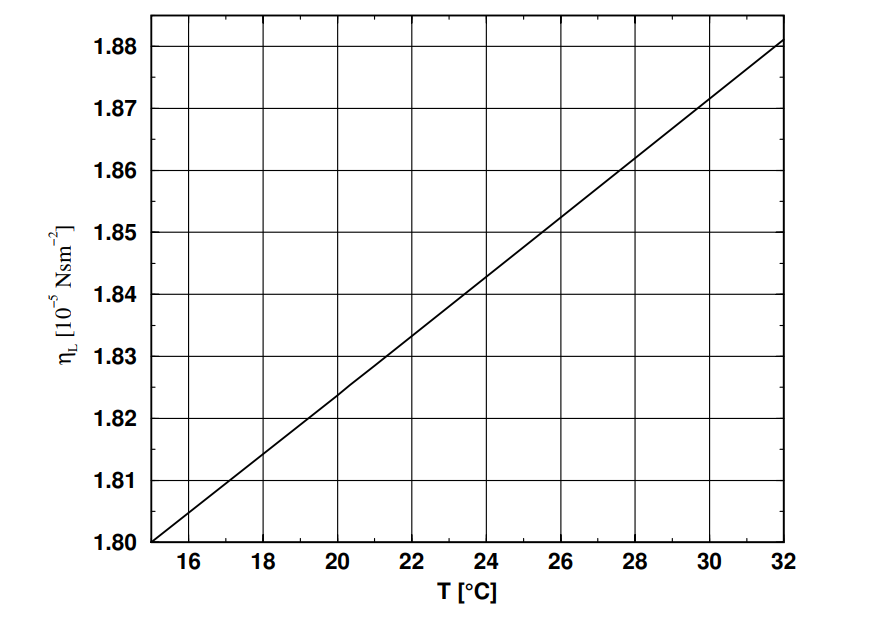
\includegraphics[width=\textwidth]{img/viskositaet.png}
  \caption{Viskosität von Luft bei verschiedenen Temperaturen \cite{V503}.}
  \label{fig:viskositaet}
\end{figure}
Damit folgt für die Werte $\in$ [1,6] eine Viskoistät von $\eta = \SI{1.85e-5}{\pascal\second}$ und für die Werte $\in$ [7,12] eine Viskosität von $\eta = \SI{1.86e-5}{\pascal\second}$.
Mit $g = \SI{9.81}{\meter\per\second\squared}$, $\rho_{\symup{Oel}} = \SI{886}{\kilo\gram\per\meter\cubed}$, $\rho_{\symup{Luft}} = \SI{1.204}{\kilo\gram\per\meter\cubed}$ und der Feldstärke $E$ folgen die Werte in \autoref{tab:ladung}. Die Feldstärke ergibt sich 
mit der angelegten Spannung $U$ und dem Plattenabstand $d = \SI{7.6250(0.0051)}{mm}$ zu $E = \frac{U}{d}$.
\begin{table}[H]
  \centering
  \caption{Ladung und Radius der Öltröpfchen.}
  \label{tab:ladung}
  \begin{tabular}{c | c}
    \toprule
    {$q\,/\symup{10^{-19}\,C}$} & {$r\,/\symup{10^{-7}\,m}$}\\
    \midrule
    2.97 $\pm$ 0.92 & 7.42 $\pm$ 0.74 \\
    3.78 $\pm$ 1.23 & 4.24 $\pm$ 0.52 \\
    7.49 $\pm$ 2.42 & 5.95 $\pm$ 0.72 \\
    4.99 $\pm$ 1.58 & 6.69 $\pm$ 0.74 \\
    7.16 $\pm$ 2.21 & 1.07 $\pm$ 0.10 \\
    4.81 $\pm$ 1.49 & 9.68 $\pm$ 0.97 \\
    3.01 $\pm$ 9.50 & 5.86 $\pm$ 0.59 \\
    7.26 $\pm$ 2.28 & 7.83 $\pm$ 0.81 \\
    1.76 $\pm$ 0.56 & 6.45 $\pm$ 0.67 \\
    8.72 $\pm$ 2.71 & 9.07 $\pm$ 0.91 \\
    9.50 $\pm$ 2.97 & 8.48 $\pm$ 0.87 \\
    2.89 $\pm$ 9.06 & 7.14 $\pm$ 0.72 \\
    \bottomrule
  \end{tabular}
\end{table}
Da die Öltröpfchen sehr klein sind und das Gesetz von Stokes nur für Tröpfchen gilt deren Abmessungen groß gegenüber der mittleren freien Weglänge der Luftmoleküle sind, wird die Korrektur nach Cunningham verwendet.
Die Korrektur ist gegeben durch
\begin{equation*}
  \eta_{\symup{eff}} = \eta_{\symup{Luft}} \cdot \left(1 + \frac{B}{p \cdot r}\right)^{-1},
\end{equation*}
mit dem Druck $p$ und dem Cunningham-Korrekturfaktor $B$. Für die Berechnung wird der Druck auf Normaldruck $p = \SI{101325}{Pa}$ gesetzt. Der Cunningham-Korrekturfaktor ist gegeben durch 
$B = \SI{0.0082259674}{Pa\,m}$ \cite{V503}. Damit ergibt sich auch eine korrigierte Ladung in \autoref{eq:korrigierte_ladung}. Die korrigierten Werte für die Viskosität und Ladung sind in \autoref{tab:viskositaet_eff} zu sehen.
\begin{table}[H]
  \centering
  \caption{Korrigierte Viskosität von Luft.}
  \label{tab:viskositaet_eff}
  \begin{tabular}{c | c}
    \toprule
    {$\eta_{\symup{eff}}\,/\symup{10^{-5}\,Pa\,s}$} & {$q_{\symup{eff}}\,/\symup{10^{-19}\,C}$}\\
    \midrule
    1.66 $\pm$ 0.05 & 2.97 $\pm$ 0.92 \\
    1.55 $\pm$ 0.05 & 3.78 $\pm$ 1.23 \\
    1.62 $\pm$ 0.05 & 7.49 $\pm$ 2.42 \\
    1.64 $\pm$ 0.05 & 4.99 $\pm$ 1.58 \\
    1.71 $\pm$ 0.04 & 7.16 $\pm$ 2.21 \\
    1.71 $\pm$ 0.04 & 4.81 $\pm$ 1.49 \\
    1.63 $\pm$ 0.05 & 3.01 $\pm$ 0.95 \\
    1.68 $\pm$ 0.05 & 7.26 $\pm$ 2.28 \\
    1.65 $\pm$ 0.05 & 1.76 $\pm$ 5.61 \\
    1.70 $\pm$ 0.04 & 8.72 $\pm$ 2.71 \\
    1.69 $\pm$ 0.04 & 9.50 $\pm$ 2.97 \\
    1.67 $\pm$ 0.05 & 2.89 $\pm$ 9.06 \\
    \bottomrule
  \end{tabular}
\end{table}
Mit python wird der größte gemeinsame Teiler der Ladungen berechnet. Dieser ist $e_{exp} = \SI{1.5592(0.6624)e-19}{C}$. Der größte gemeinsame Teiler wird mit einer Toleranz von
$q_{tol} = 0.2\cdot10^{-19}$ berechnet. Die Toleranz wurde so gewählt, dass der Fehler des größten gemeinsamen Teilers möglichst klein wird.
Aus dieser Berechnung lässt sich schließen, dass Ladung gequantelt auftritt. Die Ladung der Öltröpfchen ist also ein ganzzahliges Vielfaches der Elementarladung $e_{exp}$.\\
\\
Die korrigierte Ladung wird nun in \autoref{fig:ladung} aufgetragen. Die Schritte auf der y-Achse sind dabei $\SI{1.602e-19}{C}$. Auf der x-Achse ist der Index der akzeptierten
Werte aufgetragen. Die Fehlerbalken sind ebenfalls eingezeichnet.

\begin{figure}[H]
  \centering
  \includegraphics[width=\textwidth]{build/plot1.pdf}
  \caption{Ladung der Öltröpfchen.}
  \label{fig:ladung}
\end{figure}

Auch hier ist zu erkennen, dass die Ladung, größtenteils, gequantelt auftritt. Zu erkennen ist jedoch auch, dass einige Werte nicht ganzzahlige Vielfache der Elementarladung sind.

\subsection{Bestimmung der Avogadro-Konstante}
Die Avogadro-Konstante wird mit
\begin{equation*}
  N_A = \frac{F_c}{e_{exp}}
\end{equation*}
bestimmt. Dabei ist $F_c$ die Faraday-Konstante.
Somit ergibt sich mit $F_C = \SI{9.648e+04}{C\per\mol}$ \cite{faraday} und $e_{exp} = \SI{1.5592(0.6624)e-19}{C}$ die Avogadro-Konstante zu 
\begin{equation*}
  N_A = \SI{6.1883(2.6)e23}{\per\mol}.
\end{equation*}

\newpage